\chapter{Evaluation} % (fold)
\label{cha:evaluation}

\section{Evaluation Methodology} % (fold)
\label{sec:evaluation:evaluation_methodology}

This chapter present the results of each technique described on Chapter \ref{cha:tracking_library_for_the_web}. Two metrics were utilized to analyze the solutions available on \textit{tracking.js} library:

\begin{enumerate}
	\item Frames per second (FPS): present FPS metric of how the implemented techinques performs on the web environment in order to reach real-time capability. On the United Kingdom popular video format known as Phase Alternating Line (PAL) \cite{PAL1962}, real time video is represented by 25 FPS, therefore this value is used to define whether the tests can or cannot be considered real-time.
	\item Partial occlusion robustness: present tests how the implemented techinques reacts to partial occlusions.
\end{enumerate}

In addition to the two metrics described above, a comparison between \textit{tracking.js} and existing solutions involving server-side tracking is presented \cite{Pablo2013}, showing benefits of a pure JavaScript client-side tracking solution.
All tests were executed on Google Chrome browser version 28.0.1500.71 \cite{Chrome2010}, running on Mac OS X 10.8.3, 2.6 GHz Intel Core i7 16 GB 1600 MHz RAM.

% section evaluation_methodology (end)

\section{Results} % (fold)
\label{sec:evaluation:results}

\subsection{Rapid Object Detection (Viola Jones)} % (fold)
\label{sec:evaluation:results:rapid_object_detection}

\subsubsection{Discussion} % (fold)
\label{subsub:evaluation:results:rapid_object_detection:discussion}

Having Viola Jones rapid object detection as part of the library resulted in interesting examples for web applications, such as detecting faces, mouths, eyes and any other training data \cite{Viola2001}. On Figure \ref{figure:viola_overview} is shown different examples of training data being used by the library implementation of Viola Jones.

\begin{figure}[!htb]
  \centering
  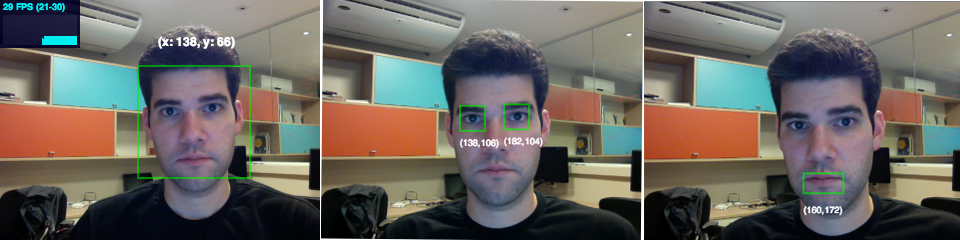
\includegraphics[width=\linewidth]{chapters/evaluation/viola_overview.png}
  \caption{Library implementation of Viola Jones using different training datas for detecting faces, eyes and mouth.}
  \label{figure:viola_overview}
\end{figure}

\begin{figure}[!htb]
  \centering
  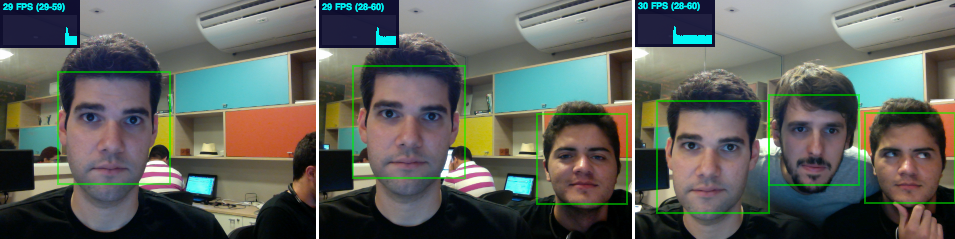
\includegraphics[width=\linewidth]{chapters/evaluation/viola.png}
  \caption{Library implementation of Viola Jones detecting multiple faces inside the real-time limit of 25 FPS.}
  \label{figure:viola_multiple_faces}
\end{figure}

Augmented reality and tracking applications for advertising and entertainment are gaining more space on the web enviroment. The media used in this kind of application needs to be as appealing as possible in order to catch consumers' attention, thus detecting faces, or augmenting the scene with objects are attractive possibilities. In order to demonstrate that concept, a simple chat application was created. In this chat application, while talking in real-time, the users could augment their faces with objects, such as a fake glass with mustache. In order to extract the users eyes coordinates Viola Jones was used. Listing \ref{lst:viola} shows the simplified JavaScript API provided by \textit{tracking.js} in order to extract eyes coordinates and draw the image. The fake glasses are positioned over $x$ and $y$ coordinates on the canvas axis based on the extracted values. Figure \ref{figure:viola_glass_face} demonstrates the described example.

\begin{figure}[!htb]
  \centering
  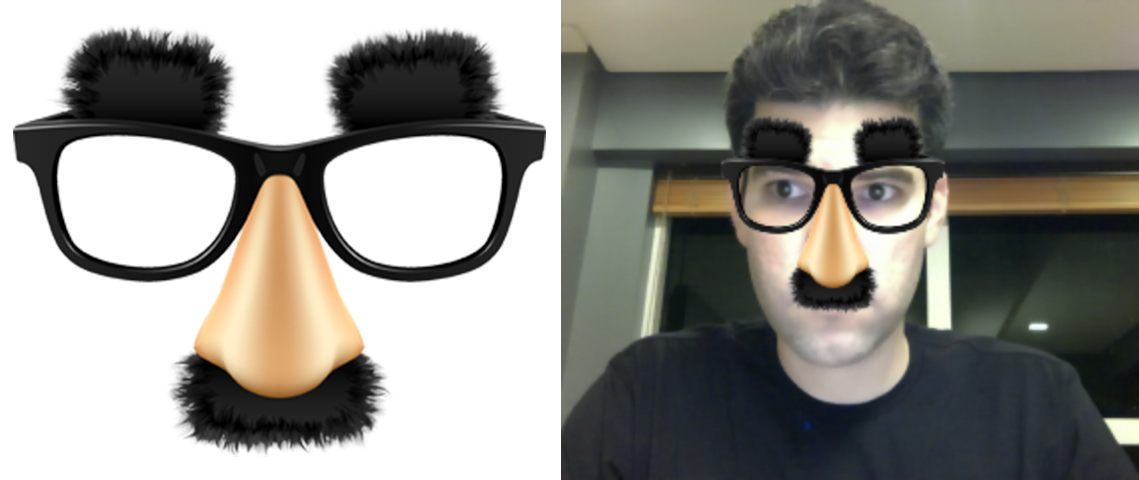
\includegraphics[width=380pt]{chapters/evaluation/viola_glass_face.png}
  \caption{Augmenting users faces with objects using \textit{tracking.js} Viola Jones eyes detection.}
  \label{figure:viola_glass_face}
\end{figure}

\begin{lstlisting}[language=C++,label={lst:viola},caption=Example of \textit{tracking.js} API of augmenting users faces with objects using Viola Jones eyes detection.]
  var img = new Image();
  img.src = 'img/glasses.png';
  var videoCamera = new tracking.VideoCamera();
  videoCamera.track({
      type: 'human',
      data: 'frontal_face',
      onFound: function(track) {
          videoCamera.canvas.context.drawImage(img, track[0].x, track[0].y, track[0].size, track[0].size);
      }
  });
\end{lstlisting}

% subsubsection discussion (end)

\subsubsection{FPS} % (fold)
\label{subsub:evaluation:results:rapid_object_detection:fps}

The United Kingdom popular video format known as Phase Alternating Line (PAL) \cite{PAL1962} defines that real time video is represented by 25 FPS, therefore this value is used to define whether the tests can or cannot be considered real-time. On Figure \ref{figure:viola_fps}, the Viola Jones implementation were tested with different numbers of detected faces. Fifteen faces were gradually added, for each addition the FPS average was recorded. Note that, until five faces detected the web implementation still runs inside the real-time limit defined by PAL \cite{PAL1962}.

\begin{figure}[!htb]
  \centering
    \begin{tikzpicture}
    \begin{axis}[
        enlarge x limits=0.03,
        minor tick num=1,
        xlabel=Number of detected faces,
        ylabel=Frames per second (FPS)]

        \addplot[wblue,mark=x] coordinates {
             (1,30)
             (2,29)
             (3,30)
             (4,27)
             (5,25)
             (6,20)
             (7,17)
             (8,16)
             (9,16)
             (10,15)
             (11,15)
             (12,13)
             (13,11)
             (14,9)
             (15,8)
         };

         \draw [red] ({rel axis cs:0,0}|-{axis cs:15,25}) -- ({rel axis cs:1,0}|-{axis cs:15,25}) node [pos=0.0, above] {};
    \end{axis}
    \end{tikzpicture}
   \caption{Library implementation of Viola Jones tested with different numbers of detected faces.}
   \label{figure:viola_fps}
\end{figure}

% subsubsection fps (end)

\subsubsection{Oclusion Robustness} % (fold)
\label{subsub:evaluation:results:rapid_object_detection:occlusion_robustness}

Viola Jones implementation of \textit{tracking.js} shows good results for partial occlusions. Figure \ref{figure:viola_occlusion} demonstrates occlusions variations that still allows the face to be detected.

\begin{figure}[!htb]
  \centering
  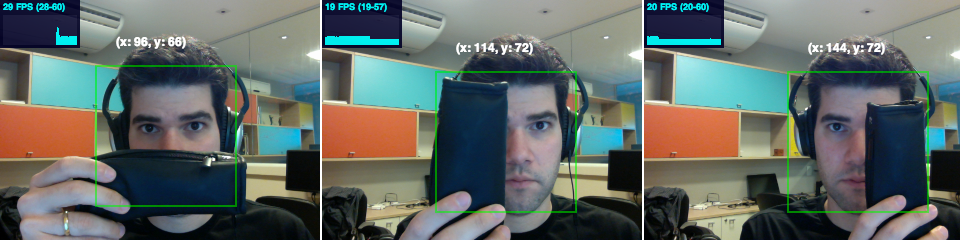
\includegraphics[width=\linewidth]{chapters/evaluation/viola_occlusion.png}
  \caption{Library implementation of Viola Jones partial occlusion robustness.}
  \label{figure:viola_occlusion}
\end{figure}

% subsubsection occlusion_robustness (end)

% subsection rapid_object_detection (end)

\subsection{Color Tracking Algorithm} % (fold)
\label{sec:evaluation:results:color_tracking_algorithm}

\subsubsection{Discussion} % (fold)
\label{subsub:evaluation:results:color_tracking_algorithm:discussion}

Being able to use colored objects to control your browser using the user camera is very appealing. Any colored object could be used to enable user interaction with your web application using \textit{tracking.js} color tracking technique trough a simple and intuitive JavaScript API. On Figure \ref{figure:color_object} is shown different colored objects being tracked.

\begin{figure}[!htb]
  \centering
  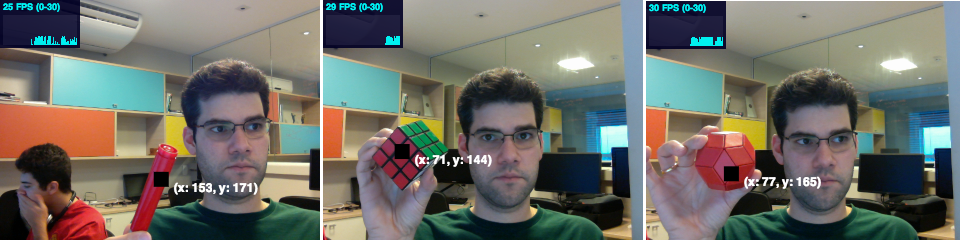
\includegraphics[width=\linewidth]{chapters/evaluation/color_object.png}
  \caption{Library implementation of color tracking for different objects: On the left a red pencil marker; on the center a Rubik's magic cube \cite{Rubiks2013} from the red face; and on the right a red Ball of Whacks \cite{Whack2013}.}
  \label{figure:color_object}
\end{figure}

Enable entertainment web applications is also possible using color tracking. Few examples were implemented using color tracking and a PlayStation move controller (Figure \ref{figure:psmove}) that is basically a colored sphere that can emit light, the color of the sphere can be set via Bluetooth. This controller have four buttons, square, triangle, cross, circle, which are color coded as pink, green, blue and red. The controller has also three types of built-in sensors, temperature, accelerometer, gyroscope and magnetometer. In this work only the emitted light is used to track the scene.

\begin{figure}[!htb]
  \centering
  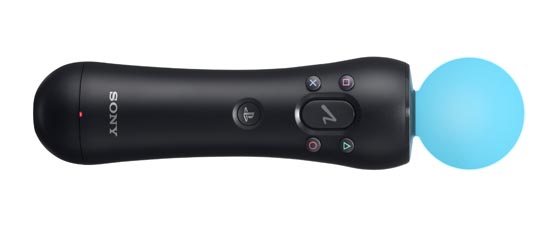
\includegraphics[width=280pt]{chapters/evaluation/psmove.png}
  \caption{PlayStation move controller.}
  \label{figure:psmove}
\end{figure}

On Figure \ref{figure:color_games}, the two bottom images are examples of how games could be developed to the web trough color tracking. On the bottom left, a multi-player game that allows the user to draw in order to competitors guess what is the drawing meaning is demonstrated. On the bottom right, multiple PlayStation move controllers are used to control the user interactions into a 3D environment rendered trough the GPU using WebGL \cite{WebGL2013}. Note that, the available \textit{tracking.js} techniques could be combined with WebGL rendering in order to reach real-time 3D rendering.

\begin{figure}[!htb]
  \centering
  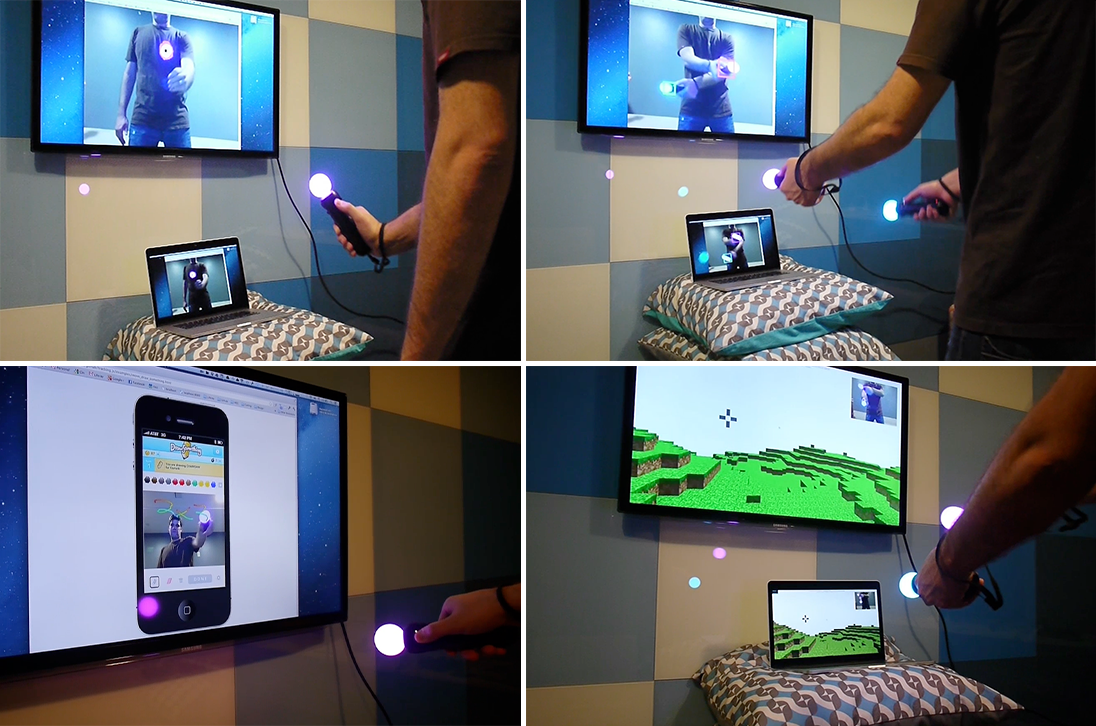
\includegraphics[width=\linewidth]{chapters/evaluation/color_games.png}
  \caption{Library implementation of color tracking used in games running on the web. On the Bottom left, a multi-player game that allows the user to draw using the camera. On the bottom right, multiple PlayStation move controllers are used to control the user interactions into a 3D environment.}
  \label{figure:color_games}
\end{figure}

Another example of color tracking on user interactions is demonstrated on Figure \ref{figure:color_volume}. Using a HTML5 audio element \cite{International2009} a music is played and trough any colored object, the user can control the volume of the player sliding the object from the left to right, left most coordinates means volume set to zero, right most coordinates means volume set to maximum.

\begin{figure}[!htb]
  \centering
  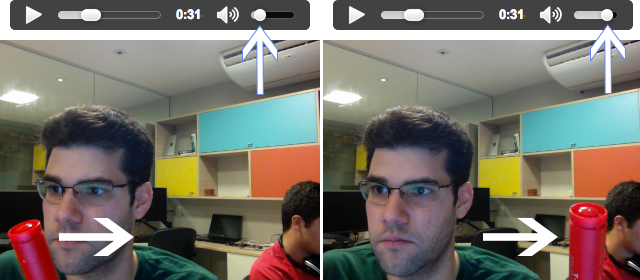
\includegraphics[width=\linewidth]{chapters/evaluation/color_volume.png}
  \caption{Library implementation of color tracking controlling the HTML5 audio element volume.}
  \label{figure:color_volume}
\end{figure}

% subsubsection discussion (end)

\subsubsection{FPS} % (fold)
\label{subsub:evaluation:results:color_tracking_algorithm:fps}

On Figure \ref{figure:color_fps}, the color tracking implementation were tested with different numbers of pixels detected. The size of the detect object were gradually increased, resulting in a bigger number of pixels found, for each incrementation in the size the FPS average was recorded. Note that, until $2138$ pixels detected the web implementation still runs inside the real-time limit defined by PAL \cite{PAL1962}.

\begin{figure}[!htb]
  \centering
    \begin{tikzpicture}
    \begin{axis}[
        enlarge x limits=0.03,
        minor tick num=1,
        xlabel=Number of pixels detected,
        ylabel=Frames per second (FPS)]

        \addplot[wblue,mark=x] coordinates {
        (174,30)
        (178,30)
        (178,30)
        (172,30)
        (164,30)
        (164,30)
        (150,30)
        (150,30)
        (156,30)
        (192,30)
        (192,30)
        (200,30)
        (200,30)
        (184,30)
        (160,30)
        (160,30)
        (160,30)
        (160,30)
        (158,30)
        (158,30)
        (162,30)
        (162,30)
        (180,30)
        (160,30)
        (160,30)
        (154,30)
        (154,30)
        (162,30)
        (162,30)
        (194,30)
        (194,29)
        (172,29)
        (172,29)
        (182,29)
        (134,29)
        (134,29)
        (160,29)
        (160,29)
        (176,29)
        (176,29)
        (154,29)
        (154,29)
        (184,29)
        (184,29)
        (172,29)
        (182,29)
        (182,29)
        (164,29)
        (164,29)
        (148,29)
        (148,29)
        (122,29)
        (122,29)
        (122,29)
        (138,29)
        (138,29)
        (162,29)
        (162,29)
        (176,29)
        (176,29)
        (208,30)
        (208,30)
        (208,30)
        (208,30)
        (200,30)
        (202,30)
        (202,30)
        (194,30)
        (194,30)
        (198,30)
        (198,30)
        (246,30)
        (246,30)
        (308,30)
        (308,30)
        (274,30)
        (254,30)
        (254,30)
        (322,30)
        (322,30)
        (406,30)
        (406,30)
        (434,30)
        (434,30)
        (408,30)
        (412,30)
        (470,30)
        (478,30)
        (478,30)
        (478,30)
        (546,29)
        (668,29)
        (668,29)
        (660,29)
        (700,29)
        (700,29)
        (756,29)
        (756,29)
        (848,29)
        (848,29)
        (890,29)
        (890,29)
        (884,29)
        (884,29)
        (880,29)
        (914,29)
        (914,29)
        (910,29)
        (910,29)
        (934,29)
        (934,29)
        (908,29)
        (908,29)
        (898,29)
        (974,29)
        (974,29)
        (998,29)
        (998,29)
        (1016,29)
        (1016,29)
        (1100,30)
        (1100,30)
        (1044,30)
        (1044,30)
        (1090,30)
        (1074,30)
        (1074,30)
        (1160,30)
        (1160,30)
        (1170,30)
        (1170,30)
        (1222,30)
        (1222,30)
        (1160,30)
        (1160,30)
        (1216,30)
        (1170,30)
        (1170,30)
        (1108,30)
        (1108,30)
        (1110,30)
        (1110,30)
        (1148,30)
        (1148,30)
        (1158,30)
        (1140,30)
        (1140,30)
        (1202,30)
        (1232,30)
        (1232,29)
        (1342,29)
        (1342,29)
        (1362,29)
        (1472,29)
        (1548,29)
        (1638,29)
        (1638,29)
        (1762,29)
        (1822,29)
        (1822,29)
        (1814,29)
        (1850,29)
        (1880,29)
        (1880,29)
        (1856,29)
        (1854,29)
        (1854,29)
        (1974,29)
        (1980,29)
        (1992,29)
        (2076,29)
        (2138,29)
        (2138,23)
        (2202,23)
        (2288,23)
        (2288,23)
        (2366,23)
        (2366,23)
        (2386,23)
        (2432,23)
        (2466,23)
        (2466,23)
        (2548,23)
        (2632,23)
        (2632,23)
        (2692,23)
        (2738,23)
        (2742,23)
        (2742,23)
        (2854,23)
        (2812,23)
        (2812,23)
        (2852,19)
        (2856,19)
        (2914,19)
        (2914,19)
        (2974,19)
        (2974,19)
        (2976,19)
        (3042,19)
        (3026,19)
        (3080,19)
        (3090,19)
        (3146,19)
        (3130,19)
        (3142,19)
        (3142,19)
        (3156,19)
        (3186,19)
        (3198,19)
        (3208,19)
        (3218,18)
        (3220,18)
        (3220,18)
        (3286,18)
        (3316,18)
        (3376,18)
        (3370,18)
        (3392,18)
        (3404,18)
        (3408,18)
        (3442,18)
        (3450,18)
        (3492,18)
        (3516,18)
        (3518,18)
        (3516,18)
        (3512,15)
        (3502,15)
        (3524,15)
        (3546,15)
        (3550,15)
        (3560,15)
        (3586,15)
        (3616,15)
        (3654,15)
        (3692,15)
        (3692,15)
        (3718,15)
        (3766,15)
        (3820,15)
        (3824,15)
        (3852,15)
        (3894,15)
        (3948,15)
        (3988,15)
        (4024,15)
        (4068,15)
        (4150,15)
        (4314,15)
        (4500,15)
        (4612,15)
        (4670,15)
        (4784,15)
        (4894,15)
        (4912,15)
        (4920,13)
        (4994,13)
        (5062,13)
        (5160,13)
        (5218,13)
        (5230,13)
        (5378,13)
        (5404,13)
        (5494,13)
        (5590,13)
        (5626,13)
        (5734,11)
        (5816,11)
        (5942,11)
        (6108,11)
        (6278,11)
        (6370,11)
        (6450,11)
        (6528,11)
        (6770,11)
        (6806,9)
        (7040,9)
        (7246,9)
        (7448,9)
        (7698,9)
        (7788,9)
        (7846,9)
        (7882,7)
        (7940,7)
        (7996,7)
        (8012,7)
        (7966,7)
        (7412,7)
         };

         \draw [red] ({rel axis cs:0,0}|-{axis cs:15,25}) -- ({rel axis cs:1,0}|-{axis cs:15,25}) node [pos=0.0, above] {};
    \end{axis}
    \end{tikzpicture}
   \caption{Library implementation of color tracking technique tested with different numbers of pixels detected.}
   \label{figure:color_fps}
\end{figure}

% subsubsection fps (end)

\subsubsection{Oclusion Robustness} % (fold)
\label{subsub:evaluation:results:color_tracking_algorithm:occlusion_robustness}

Color tracking technique implementation of \textit{tracking.js} shows good results for partial occlusions. Figure \ref{figure:color_occlusion} demonstrates occlusions variations that still allows the face to be detected.

\begin{figure}[!htb]
  \centering
  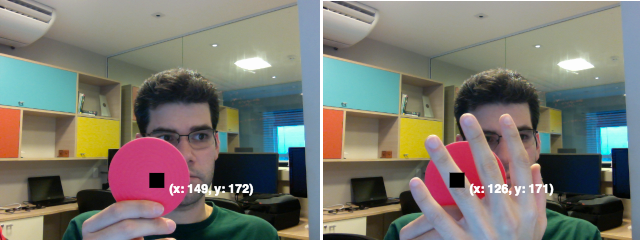
\includegraphics[width=\linewidth]{chapters/evaluation/color_occlusion.png}
  \caption{Library implementation of color tracking technique partial occlusion robustness.}
  \label{figure:color_occlusion}
\end{figure}

% subsubsection occlusion_robustness (end)

% subsection color_tracking_algorithm (end)

\subsection{Markerless Tracking Algorithm} % (fold)
\label{sec:evaluation:results:markerless_tracking_algorithm}

\subsubsection{Matching Robustness} % (fold)
\label{subsub:evaluation:results:markerless_tracking_algorithm:matching_robustness}

Lorem ipsum dolor sit amet, consectetur adipisicing elit.

% subsubsection matching_robustness (end)

\subsubsection{Oclusion Robustness} % (fold)
\label{subsub:evaluation:results:markerless_tracking_algorithm:occlusion_robustness}

Lorem ipsum dolor sit amet, consectetur adipisicing elit.

% subsubsection occlusion_robustness (end)

% subsection markerless_tracking_algorithm (end)

% section results (end)

% chapter evaluation (end)